

\chapter{Information Theory and Rate Distortion Theory}
\label{ch01}


\section{Introduction}
\label{ch01.sec.11.1}

Thus far in the book, the term \textit{information}
has been used sparingly and when
it has been used, we have purposely been imprecise as to its meaning.
Although,
everyone  has an intuitive feeling for what information is,
it is difficult to attach
a meaningful quantitative definition to the term. In the context of
communication systems, Claude Shannon was able to do exactly this,
and as a result, opened up an entirely new view of communication systems
analysis and design~\cite{Levin2002}.
The principal contribution of Shannon's information theory to date has been
to allow communication theorists to establish absolute
bounds on communication systems performance that cannot be exceeded no matter
how ingeniously designed or complex our communication systems are.
Fundamental physical limitations on communication systems performance is
another topic that has been largely ignored in the preceding chapters,
\textbf{(OBS: mentions preceding chapters.)}
but it is a subject of exceptional practical importance.
For example, for any of the numerous communication systems developed
thus far in the book, we could decide to design
a new system that would outperform the accepted standard for a particular
application. The first question that we should ask is: how close is the
present system to achieving theoretically optimum performance?
If the existing communication system operates at or near the fundamental
physical limit on performance, our task may be difficult or impossible.
However, if the existing system is far away from the absolute
performance bound, this might be an area for fruitful work.

Of course, in specifying the particular communication system under
investigation, we must know the important physical parameters,
such as transmitted
power, bandwidth, type(s) of noise present, and so on,
and information theory allows these constraints to be incorporated.
However, information theory does not provide a way for communication system
complexity to be explicitly included.
Although, this is something of a drawback, information theory itself provides
a way around this difficulty, since it is generally true that as we approach
the fundamental limit on the performance of a communication system,
the system complexity increases, sometimes quite drastically.
Therefore, for a simple communication system operating far
from its performance bound, we may be able to improve the performance
with a relatively modest increase in complexity.
On the other hand, if we have a rather complicated communication system
operating near its fundamental limit, any performance improvement may
be possible only with an extremely complicated system.

In this chapter we are concerned with the rather general block diagram
shown in Fig.~\ref{ch01.fig11.1.1}. Most of the early work by
Shannon and others ignored the source  encoder/decoder blocks and
concentrated  on bounding the performance of the channel
encoder/decoder pair. Subsequently, the source  encoder/decoder blocks
have attracted much research attention.  In this chapter we consider
both topics and expose the reader to the nomenclature used in the
information theory literature.
Quantitative definitions of information are presented in
Sec.~\ref{ch01.sec11.2} that lay the foundation for the remaining
sections. In Secs.~\ref{ch01.sec11.3} and~\ref{ch01.sec11.4} we present
the fundamental source and channel coding theorems, give some examples,
and state the implications of these theorems.
Section~\ref{ch01.sec11.5} contains a brief development of rate
distortion theory,
which is the mathematical basis for data compression.
A few applications of the theory in this chapter are presented
in Sec.~\ref{ch01.sec11.6}, and a technique for variable-length
source coding is given in Sec.~\ref{ch01.sec11.7}.


\begin{figure}[hbt] % 01
  \centering
  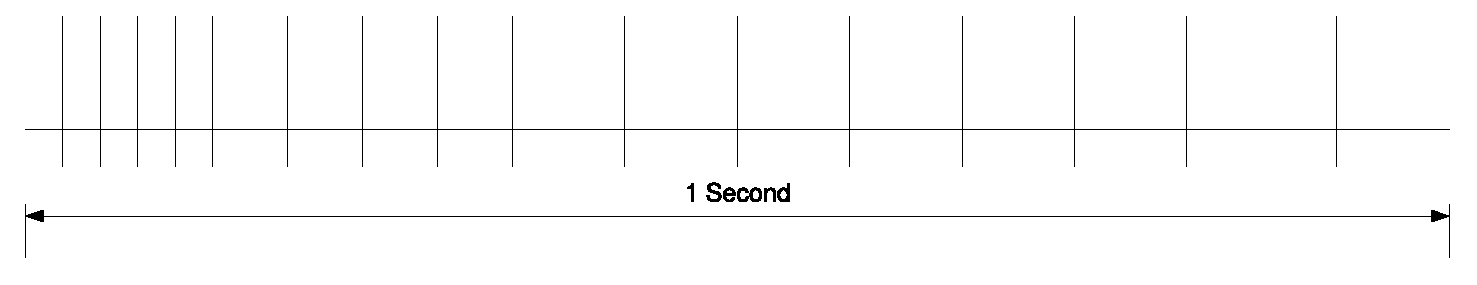
\includegraphics[width=3.3in]{line-spaces.eps}
\caption{Communication system block diagram.
\label{ch01.fig11.1.1} }
\end{figure}


\section{Entropy and Average Mutual Information}
\label{ch01.sec11.2}

Consider a discrete random variable $U$ that takes on
the values $\{u_1, u_2, \dots, u_M\}$, where the set of possible
values of $U$ is often called the \textit{alphabet} and the elements
of the set are called \textit{letters} of the alphabet. Let $P_U(u)$
denote the probability  assignment  over the alphabet, then we can
define the \textit{self-information} of the event $ u = u_j $ by
\begin{equation}
  I_U \left( u_j \right) = \log \frac{1}{P_U (u_j)} = - \log P_U
    \left( u_j \right)~.
\label{ch01.eq11.2.1}
\end{equation}
The quantity $I_U (u_j) $ is a measure  of the information  contained
in the event $ u = u_j$. Note that the base of the logarithm in
Eq.~\eqref{ch01.eq11.2.1} is unspecified. It is common
to use base $e$, in which case $I_U (\cdot) $ is in natural units (nats),
or base 2,  in which case $I_U(\cdot)$ is in binary units (bits).
Either base is acceptable since the difference in the two bases is just a
scaling operation. We will use base 2 in all of our work,
and hence $I_U(\cdot)$ and related quantities will be in bits.
The average or expected value of the self-information is called the
\textit{entropy,} also discrete entropy or absolute entropy, and is given by
\begin{equation}
 \displaystyle H(U) = - \sum^M_{j=1} P_U \left(u_j\right)
    \log P_U \left(u_j \right)~.
\label{ch01.eq11.2.2}
\end{equation}
The following example illustrates the calculation of entropy and how it is
affected by probability assignments.

\begin{example}
\label{ch01.ex11.2.1}
Given a random variable $U$ with four equally likely letters
in its alphabet, we wish to find $H(U)$. Clearly, $M=4$
and $P_U(u_i)= \tfrac{1}{4}$ for $ i = 1, 2, 3, 4 $. Thus, from
Eq.~\eqref{ch01.eq11.2.2},
\begin{align}
 H(U) \displaystyle & = - \sum^4_{j=1} \tfrac{1}{4} \log \tfrac{1}{4}
 \notag\\
 \displaystyle & = - \log \tfrac{1}{4} = 2 \textrm{ bits}~.
\label{ch01.eq11.2.3}
\end{align}
We now consider a discrete random  variable $X$ with four letters such that
$P_X (x_1) = \tfrac{1}{2},
 P_X (x_2) = \tfrac{1}{4},
 P_X (x_3) = P_X (x_4) = \tfrac{1}{8} $.
Again, we wish to find the entropy of this random variable. Directly,
\begin{equation}
 H(X)
 = -
 \tfrac{1}{2} \log
 \tfrac{1}{2} -
 \tfrac{1}{4} \log
 \tfrac{1}{4} -
 \tfrac{1}{8}
 \log
 \tfrac{1}{8} -
 \tfrac{1}{8}
 \log
 \tfrac{1}{8}
 = 1.75 \textrm{ bits}~.
\label{ch01.eq11.2.4}
\end{equation}
Comparing Eqs.~\eqref{ch01.eq11.2.3} and~\eqref{ch01.eq11.2.4}, we see
that equally likely letters produce a larger entropy.
This result is true in general, as we will see shortly.
\end{example}

We now consider two jointly distributed discrete random variables $W$ and
$X$with the probability assignment
$P_{WX} (w_j, x_k), j = 1,2,\dots, M, k = 1,2,\dots, N$.
We are particularly interested in the interpretation that $w$ is an
input letter to a noisy channel and $x$ is the corresponding output.
The information provided about the event $w=w_j$ by the occurrence of the
event $x=x_k$ is
\begin{equation}
 I_{W;X} \left(w_j;x_k\right)
   = \log \frac{P_{W|X} \left(w_j|x_k\right)} {P_W \left(w_j\right)}~.
\label{ch01.eq11.2.5}
\end{equation}
Further, the information provided about the event $x=x_k$ by the occurrence of
$w= w_j$ is
\begin{equation}
 I_{X ; W} \left( x_k; w_j \right) =\log
  \frac{P_{X|W} \left( x_k| w_j\right)}  {P_X \left(x_k\right)} ~.
\label{ch01.eq11.2.6}
\end{equation}
We can show that $ I_{W;X}(w_j;x_k) =  I_{X;W}(x_k; w_j)$ by starting with
Eq.~\eqref{ch01.eq11.2.5} and using conditional probability as follows:
\begin{align}
    I_{W;X}\left(w_j;x_k\right)
    & = \log
    \frac{P_{WX}\left(w_j, x_k\right)}{P_W\left(w_j\right)
              P_X\left(x_k\right)}
    \notag\\
    & = \log
    \frac{P_{X|W} \left( x_k | w_j\right)} {P_X \left(x_k\right)}
    =
     I_{X;W} \left(x_k; w_j\right) ~.
\label{ch01.eq11.2.7}
\end{align}
Because of this symmetry,
Eqs.~\eqref{ch01.eq11.2.5} and~\eqref{ch01.eq11.2.6}
are called  the \textit{mutual information}
between the events $w= w_j $ and $x= x_k$.
The \textit{average mutual information}
over the joint ensemble is an important quantity defined by
\begin{align}
 I(W;X) & \displaystyle = \sum^M_{j=1} \, \sum^N_{k=1} P_{WX}
 \left(w_j, x_k\right) I_{W;X} \left(w_j; x_k\right)
 \notag\\
 &\displaystyle = \sum^M_{j=1} \, \sum^N_{k=1} P_{WX}
 \left(w_j, x_k\right) \log
 \frac{ P_{W |X} \big(w_j |  x_k\big)}{P_W\left(w_j\right)}~.
\label{ch01.eq11.2.8}
\end{align}
By a straightforward manipulation of Eq.~\eqref{ch01.eq11.2.5},
\begin{align}
 I_{W;X} \big(w_j;x_k\big) & = - \log P_W \big(w_j\big) +
 \log P_{W|X} \big(w_j|x_k\big)
 \notag\\
 & =  I_W \big(w_j\big) - I_{W|X} \big(w_j| x_k\big)~,
\label{ch01.eq11.2.9}
\end{align}
where
\begin{equation}
        I_{W|X} \big(w_j | x_k \big) \stackrel{\triangle}{=}
        - \log
        P_{W|X} \big(w_j|x_k\big)
\label{ch01.11.2.10}
\end{equation}
is called the \textit{conditional self-information,} and is interpreted
as the information that must be supplied to an observer to specify $w= w_j$
after the occurrence of $x=x_k$.
Substituting Eq.~\eqref{ch01.eq11.2.9} into Eq.~\eqref{ch01.eq11.2.8},
we find that
\begin{equation}
  I(W;X) = H(W) - H(W|X)~,
\label{ch01.eq11.2.11}
\end{equation}
where $ H(W|X) $ is the \textit{average conditional self-information.}
Since entropy is a measure of uncertainty, we see from
Eq.~\eqref{ch01.eq11.2.11} that the average mutual information can be
interpreted as the average amount of uncertainty remaining after the
observation of $X$.


\begin{example}
\label{ch01.ex11.2.2}
Here we wish to calculate the mutual information and the average
mutual information for the probability assignments
(with $M=2$ and $N=2$)
\begin{equation}
 P_W \big(w_1\big) = P_W \big(w_2\big) = \tfrac{1}{2}
\label{ch01.eq11.2.12}
\end{equation}
and
\begin{align}
 P_{X|W} \big(x_1| w_1\big) & = P_{X|W} \big(x_2| w_2\big) = 1-p
\label{ch01.eq11.2.13} \\
 P_{X|W} \big(x_1| w_2\big) & = P_{X|W} \big(x_2| w_1\big)  = p~.
\label{ch01.eq11.2.14}
\end{align}
If we interpret $W$ as the input to a channel $X$ as the output, the
transition probabilities in Eqs.~\eqref{ch01.eq11.2.13}
and~\eqref{ch01.eq11.2.14} are representative of what is called a
\textit{binary symmetric channel} (BSC).

To calculate the mutual information, we could use either
Eq.~\eqref{ch01.eq11.2.5} or~\eqref{ch01.eq11.2.6}.
From the probabilities given, Eq.~\eqref{ch01.eq11.2.6} seems to be
slightly simpler. Thus, we need
$P_X (x_1)$  and $P_X (x_2)$. Directly,
\begin{align}
 P_{WX} \big(w_1,x_1\big) & = P_{X|W} \big(x_1|w_1\big) P_W \big(w_1\big) =
 \frac{1-p}{2}
 \notag\\
 &= P_{WX} \big(w_2, x_2\big)
\label{ch01.eq11.2.15}
\end{align}
and
\begin{align}
 P_{WX} \big(w_1, x_2\big) & = P_{X|W} \big(x_2 | w_1\big) P_W \big(w_1\big)
 \notag\\
  & = \frac{p}{2} = P_{WX} \big(w_2, x_1\big)~.
\label{ch01.eq11.2.16}
\end{align}
Thus,
\begin{align}
 P_X \big(x_1\big) & = P_{WX} \big(w_1, x_1\big) + P_{WX} \big(w_2, x_1\big)
 \notag\\
  & = \tfrac{1}{2} = P_X \big(x_2\big)~,
\label{ch01.eq11.2.17}
\end{align}
so the four mutual information values are
\begin{equation}
 I_{X;W}\big(x_1; w_1\big)  = \log 2(1-p) = I_{X;W} \big(x_2; w_2\big)
\label{ch01.eq11.2.18}
\end{equation}
and
\begin{equation}
 I_{X;W}\big(x_1 ; w_2\big)  = \log 2p = I_{X;W} \big(x_2; w_1\big) ~.
\label{ch01.eq11.2.19}
\end{equation}

The average mutual information follows in a straightforward fashion from
Eq.~\eqref{ch01.eq11.2.8} as
\begin{align}
 I(W;X) \displaystyle & = I(X;W) = \sum^2_{j=1}\, \sum^2_{k=1}
  P_{WX}\big(w_j, x_k\big)  \log
  \frac{P_{X|W}(x_k|w_j)}{ P_X(x_k) }
\notag\\
 \displaystyle & = \frac{1-p}{2} \log 2(1-p)+ \frac{p}{2}
 \log 2p + \frac{p}{2} \log 2p +\frac{1-p}{2} \log 2 (1-p)
\notag\\
 \displaystyle & = 1 + (1-p) \log (1-p) + p \log p~.
\label{ch01.eq11.2.20}
\end{align}
The average mutual information given by Eq.~\eqref{ch01.eq11.2.20}
is plotted versus  % vs.
$p$  in Fig.~\ref{ch01.fig11.2.1}. The results of this example are discussed
more in Sec.~\ref{ch01.sec11.4} in a communications context.
\end{example}

\begin{figure}[hbt] % 02
 \figboxes
\caption{Average mutual information for a BSC with equally likely
         inputs (Ex.~\protect\ref{ch01.ex11.2.2}).
\label{ch01.fig11.2.1} }
\end{figure}

There are numerous useful properties of entropy and average mutual information.
We state two of these properties here without proof.

\begin{property}
\label{ch01.11.pro1}
Let $U$ be a random variable with possible values $\{u_1,u_2,\dots, u_M\}$.
Then
\begin{equation}
 H(U) \leq \log M
\label{ch01.eq11.2.21}
\end{equation}
with equality if and only if the values of $U$
are equally likely to occur.
\end{property}

Example~\ref{ch01.ex11.2.1} illustrates Pr.~\ref{ch01.11.pro1}.

\begin{property}
\label{ch01.11.pro2}
Let $W$ and $X$ be jointly distributed random variables.
The average mutual information between $W$ and $X$ satisfies
\begin{equation}
  I(W;X) \geq 0
\label{ch01.eq11.2.22}
\end{equation}
with equality if and only if $W$ and $X$ are statistically independent.
\end{property}


Thus, far we have defined the entropy and average mutual information only
for discrete random variables. Given an absolutely continuous random variable
$U$ with pdf $f_U(u)$ we define the \textit{differential entropy}
of $U$ as
\begin{equation}
 h(U) = - \int^\infty_{-\infty} f_U (u) \log f_U (u)\, du~.
\label{ch01.eq11.2.23}
\end{equation}
Although, Eqs.~\eqref{ch01.eq11.2.2} and~\eqref{ch01.eq11.2.23} are
functionally quite similar, there is a significant difference between
the interpretations of absolute or discrete entropy and differencial entropy.
While $H(U)$ is an absolute indicator of ``randomness,'' $h(U)$ is
only an indicator of randomness with respect to a coordinate system:
hence the names ``absolute entropy'' for $H(U)$ and ``differential entropy''
for $h(U)$.
The following example illustrates the calculation of differential entropy
and its property of indicating randomness with respect to a coordinate system.

\begin{example}
\label{ch01.ex11.2.3}
Consider an absolutely continuous random variable with uniform pdf
\begin{equation}
 f_U(u)=
 \left\{
 \begin{array}{cl}
 \displaystyle \frac{1}{a},
 & \displaystyle \frac{-a}{2} \leq u \leq \frac{a}{2}\\[2.5mm]
 \displaystyle 0, & \textrm{elsewhere}~.
 \end{array}
 \right.
\label{ch01.eq11.2.24}
\end{equation}
(1) Let $a=1$ in Eq.~\eqref{ch01.eq11.2.24} and find $h(U)$. Then
\begin{equation}
 h(U) = - \int^{1/2}_{-1/2} \log 1 \, du = 0~.
\label{ch01.eq11.2.25}
\end{equation}
(2) Let $a= 32$ and find $h(U)$. We have
\begin{equation}
 h(U) = - \int^{16}_{-16} \tfrac{1}{32}
          \log \big( \tfrac{1}{32}\big)\, du =  5~.
\label{ch01.eq11.2.26}
\end{equation}
(3) Finally, let $a = \tfrac{1}{32}$ and find $h(U)$. Here
\begin{equation}
 h(U) = - \int^{1/64}_{-1/64} 32 \log (32)\, du = - 5~.
\label{ch01.eq11.2.27}
\end{equation}
The fact that differential entropy is a relative indicator of randomness is
evident from these three special cases of the uniform distribution. Clearly,
$h(U)$ is not an absolute indicator of randomness, since in case (3) $h(U)$
is
negative, and negative randomness is difficult to interpret physically!
The ``reference''distribution is the uniform distribution over a unit
interval, with
``broader'' distributions having a positive entropy and ``narrower''
distributions having a negative differential entropy.
\end{example}

Differential entropies are unlike absolute entropy in that differential
entropy is not always
positive, not necessarily finite, not invariant to a one-to-one transformation
of the random variable, and not subject to interpretation as an average
self-information.

The average mutual information of two jointly distributed continuous random
variables, say $W$ and $X$, can also be defined as
\begin{align}
 I (W;X) &= \int^\infty_{-\infty} \,\int^\infty_{-\infty} f_{WX} (w,x)
 \log \frac{ f_{WX} (w,x) }  {f_W (w) f_X (x)} \, dw \,dx
\notag\\
 &= I (X;W)~.
\label{ch01.eq11.2.28}
\end{align}
As in the discrete case, the average mutual information can be expressed in
terms of entropies as
\begin{align}
 I (W;X) & = h (W) -  h(W|X)
\notag\\
  &= h (X) - h (X|W)~,
\label{ch01.eq11.2.29}
\end{align}
where
\begin{equation}
 h (W|X) = - \int^\infty_{-\infty} \,\int^\infty_{-\infty} f_{WX} (w,x)
 \log f_{W|X} (w|x) \, dw \,dx ~.
\label{ch01.eq11.2.30}
\end{equation}
Fortunately for our subsequent uses  of $I(W;X)$, the average
mutual information
is invariant under any one-to-one transformation of the variables,
even though
the individual differential entropies are not.

\begin{example}
\label{ch01.ex11.2.4}
In this example we compute the differential entropy of the input and the
average mutual information between the input and output of an additive
white Gaussian noise channel with zero mean and variance $ \sigma^2_c $.
The input is
also assumed to be Gaussian with zero mean and variance $ \sigma^2_s $.
Representing the channel as shown in Fig.~\ref{ch01.fig11.2.2},
we thus have that
\begin{equation}
 f_W(w) = \frac{1}{ \sqrt{2\pi} \sigma_s } e^{-w^2/2\sigma^2_s}
\label{ch01.eq11.2.31}
\end{equation}
and
\begin{equation}
 f_{X|W} (x|w) = \frac{1}{ \sqrt{2\pi} \sigma_c }
 e^{-(x-w)^2 / 2\sigma^2_c} ~.
\label{ch01.eq11.2.32}
\end{equation}

\begin{figure}[hbt] % 03
 \figboxes
\caption{Additive noise channel.
\label{ch01.fig11.2.2} }
\end{figure}

\noindent
From Eq.~\eqref{ch01.eq11.2.23} the differential entropy of the input is
\begin{align}
 h(W) & = - \int^\infty_{-\infty} f_W(w) \log f_W (w)\,dw
\notag\\
 & =  \int^\infty_{-\infty} f_W(w)
 \left\{ \log \sqrt{2\pi} \sigma_s +
 \frac{w^2}{2\sigma^2_s} \log e \right\}\,dw
\notag\\
 &= \log  \sqrt{2\pi} \sigma_s +\tfrac{1}{2} \log e =
 \tfrac{1}{2} \log 2 \pi e \sigma^2_s~.
\label{ch01.eq11.2.33}
\end{align}
To calculate the average mutual information, we choose to employ the
expression
$I(W;X) = h(X) - h(X|W)$. We already have $f_{X|W} (x|w)$, but we need
$f_X (x)$. This follows directly as
\begin{equation}
 f_X(x) = \frac{1}
 { \sqrt{2\pi} \big[ \sigma^2_s +\sigma^2_c \big]^{1/2} }
 \, e^{-x^2/2(\sigma^2_s + \sigma^2_c )}~,
\label{ch01.eq11.2.34}
\end{equation}
since the input and the noise are independent, zero-mean Gaussian processes.
By analogy with Eq.~\eqref{ch01.eq11.2.33}, we have from
Eqs.~\eqref{ch01.eq11.2.32} and~\eqref{ch01.eq11.2.34} that
\begin{equation}
 h(X) = \tfrac{1}{2} \log 2 \pi e \big[\sigma^2_s+ \sigma^2_c\big]
\label{ch01eq.11.2.35}
\end{equation}
and
\begin{equation}
 h(X|W) = \tfrac{1}{2} \log 2 \pi e \sigma^2_c~.
\label{ch01.eq11.2.36}
\end{equation}
We thus find the average mutual information to be
\begin{align}
 I(W;X) & = \tfrac{1}{2} \log 2 \pi e \big[\sigma^2_s+\sigma^2_c \big]
  - \tfrac{1}{2} \log 2 \pi e \sigma ^2_c
\notag\\
 & = \tfrac{1}{2} \log \left( 1+ \frac{\sigma^2_s}{\sigma^2_c}\right)~.
\label{ch01.eq11.2.37}
\end{align}
In Eq.~\eqref{ch01.eq11.2.37}, we see that for
$\sigma^2_s \ll \sigma^2_c , I(W;X) \cong 0 $, while if
$\sigma^2_c \rightarrow 0$, then $I(W;X) \rightarrow \infty $.
\end{example}


\section{Source Coding Theorem}
\label{ch01.sec11.3}

We now begin to interpret the quantities developed
in Sec.~\ref{ch01.sec11.2} within a communications context.
For this particular section, we consider the communication system
block diagram in Fig.~\ref{ch01.fig11.1.1} under the assumptions that the
channel is ideal (no noise or deterministic distortion) and the channel
encoder/decoder blocks are identity mappings (a straight wire connection from
input to output of each of these blocks).
We are left with a communication system block diagram consisting of a source,
source encoder, ideal channel, source decoder, and user.
Since the channel is ideal and the channel encoder and decoder are
identities, we have, with reference to Fig.~\ref{ch01.fig11.1.1}, that
$ V = W = X = Y $. A block
diagram of the simplified communication system is shown
in Fig.~\ref{ch01.fig11.3.1}.

\begin{figure}[hbt] % 04
 \figboxes
\caption{Simplified block diagram for the source coding problem.
\label{ch01.fig11.3.1} }
\end{figure}

Just what are the physical meanings of each of the components in
Fig.~\ref{ch01.fig11.3.1}?
The source is some kind of data generation device, such as a computer or
computer peripheral, which generates a discrete-valued random variable $U$ with
alphabet $ \{ u_1, u_2, \dots, u_M \} $ and probability assignment
$ P_U (\cdot) $. For the development in this section, we assume that the
successive letters produced by the source are statistically independent.
Such a source is called a \textit{discrete memoryless source} (DMS).
The ideal channel can be thought of as some perfectly operating
modem or a mass storage device that is error-free. The user is a machine or
individual that requires the data accomplish a task. With these descriptions
thus far, it is unclear why we need the source encoder/decoder blocks or what
utility they might be. The answer is that data at the output of any given
discrete source may not be in a form that  yields the minimum required
transmitted
bit rate. The following example illustrates this point.


\begin{example}[\cite{Boeringer}]
\label{ch01.ex11.3.1}
The source output is a ternary-valued random variable that takes on the
values $\{ u_1, u_2, u_3 \}$ with probabilities
$P(u_1) = 0.7, P(u_2) = 0.15 = P(u_3)$. The
source letter produced at each time instant is assumed to be independent of
the letter produced at any other time instant, so that we have a DMS. We
wish to find a binary representation of any sequence of ternary source letters
such that the source sequence can be recovered exactly (by the decoder) and
such that the average number of binary digits per source letter is a minimum.

A straightforward assignment of binary words, called a source code, is to
let $u_1$ be represented by $00, u_2$ by $10$, and $u_3$ by $11$.
This code transmits an
average of 2 bits per source letter. Since $u_1$ occurs much more often
than the
other two letters, it seems intuitive that we should use a shorter sequence to
represent $u_1$ than those used for $u_2$ and $u_3$. One such code assignment is
\begin{align*}
  & u_1 \, \rightarrow \, 0    \\
  & u_2 \, \rightarrow \, 10   \\
  & u_3 \, \rightarrow \, 11~.
\end{align*}
Since this code has the special property (called the \textit{prefix condition})
that no
binary word assignment (codeword) is a prefix of any other codeword, the
ternary source data can be uniquely recovered from its binary encoding. The
average number of bits required per source letter, denoted here by $\bar{n}$,
is thus
\begin{align}
  \bar{n} & = 1 \, \cdot \, P(u_1) +
  2 \, \cdot \, P \big(u_2\big) + 2 \,\cdot\, P\big(u_3\big)
\notag\\
 & = 0.7 + 0.3 + 0.3 = 1.3 \textrm{ bits/source letter}~.
\label{ch01.eq11.3.1}
\end{align}
This is a clear improvement over the original 2-bits/source letter code.

To try and reduce $\bar{n}$ further, we encode pairs of source letters,
which are
listed in Tab.~\ref{ch01.tab1} together with the probability of each pair.
If we now
assign a binary word to each pair of source letters as shown in the column
labeled ``codeword'' in Tab.~\ref{ch01.tab1}, we find that the average
binary codeword
length  per source  letter is.
\begin{align}
 \bar{n} & = \tfrac{1}{2} \{ 1(0.49)  + 3(0.105) + 3(0.105) + 3(0.105) +
 4(0.105) + 6(0.0225)
 \notag\\
 & \quad {} + 6(0.0225) + 6(0.0225) + 6(0.0225) \}
 \notag\\
 & = 1.1975 \textrm{ bits/source letter}~.
\label{ch01.eq11.3.2}
\end{align}

\begin{table}[hbt]
\caption{Velocity autocorrelation function corresponding to
         different states for the PSO environment.
         \label{ch01.tab1}}
\plaincenterline{\mytable
\begin{tabular}{c|c}
\bf\cb State &
\bf\cb Velocity Autocorrelation
    \upstrut{4mm}
    \\
\cw Gas &
\cw Damped exponential
    \\ 
\cy Liquid &
\cy One period damped sinusoid with single minimum
    \\
\cw Solid &
\cw Damped sinusoid with possibly multiple-oscillations
    \\ 
\end{tabular}
\emytable}
\end{table}


\begin{center}
\begin{tabular}{|c|c|}
\hline
\bf\cb State &
\bf\cb Velocity Autocorrelation
    \upstrut{4mm}
    \\
\cw Gas &
\cw Damped exponential
    \\ 
\cy Liquid &
\cy One period damped sinusoid with single minimum
    \\
\cw Solid &
\cw Damped sinusoid with possibly multiple-oscillations
    \\ 
\hline
\end{tabular}
\end{center}


\begin{center}
\begin{tabular}{|lcccccccc|}
\hline
    {{\bf\cb Bit\hspace*{50pt}}}
  & {{\bf\cb \hspace*{10pt}7\hspace*{10pt}}}
  & {{\bf\cb \hspace*{10pt}6\hspace*{10pt}}}
  & {{\bf\cb \hspace*{10pt}5\hspace*{10pt}}}
  & {{\bf\cb \hspace*{10pt}4\hspace*{10pt}}}
  & {{\bf\cb \hspace*{10pt}3\hspace*{10pt}}}
  & {{\bf\cb \hspace*{10pt}2\hspace*{10pt}}}
  & {{\bf\cb \hspace*{10pt}1\hspace*{10pt}}}
  & {{\bf\cb \hspace*{10pt}0\hspace*{10pt}}}\\
    \multicolumn{1}{|l}{{\bf\cb 0x25}}
  & \multicolumn{1}{|c|}{{\scriptsize \cy \raisebox{1.5pt}{\texttt{PORTB7}}}}
  & \multicolumn{1}{c|}{{\scriptsize \cy \raisebox{1.5pt}{\texttt{PORTB6}}}}
  & \multicolumn{1}{c|}{{\scriptsize \cy \raisebox{1.5pt}{\texttt{PORTB5}}}}
  & \multicolumn{1}{c|}{{\scriptsize \cy \raisebox{1.5pt}{\texttt{PORTB4}}}}
  & \multicolumn{1}{c|}{{\scriptsize \cy \raisebox{1.5pt}{\texttt{PORTB3}}}}
  & \multicolumn{1}{c|}{{\scriptsize \cy \raisebox{1.5pt}{\texttt{PORTB2}}}}
  & \multicolumn{1}{c|}{{\scriptsize \cy \raisebox{1.5pt}{\texttt{PORTB1}}}}
  & \multicolumn{1}{c|}{{\scriptsize \cy \raisebox{1.5pt}{\texttt{PORTB0}}}}\\
    {{\bf\cb Read/Write}}
  & {{\cw R/W}}
  & {{\cw R/W}}
  & {{\cw R/W}}
  & {{\cw R/W}}
  & {{\cw R/W}}
  & {{\cw R/W}}
  & {{\cw R/W}}
  & {{\cw R/W}}\\
    {{\bf\cb Default}}
  & {{\cy 0}}
  & {{\cy 0}}
  & {{\cy 0}}
  & {{\cy 0}}
  & {{\cy 0}}
  & {{\cy 0}}
  & {{\cy 0}}
  & {{\cy 0}}\\
\hline
\end{tabular}
\end{center}


The value in Eq.~\eqref{ch01.eq11.3.2} is slightly better than the 1.3
achieved by our second
code. The code in Tab.~\ref{ch01.tab1} is also uniquely decodable
back into the
original ternary sequence.

Although, we have not described how the binary codes were selected, it
is clear that at least in this particular case, source coding
allows the ternar
data to be represented with a smaller number of bits than one might
originally think.
Thus, the utility of the source encoder/decoder blocks in
Fig.~\ref{ch01.fig11.3.1} is~demonstrated.
\end{example}

Example~\ref{ch01.ex11.3.1} demonstrates that source coding techniques
can be useful
for reducing the bit rate required to represent (exactly) a discrete source,
and in
Sec.~\ref{ch01.sec11.7} we present a constructive technique for designing
source codes that
is due to Huffman et al.~(2005). It is also important to note that in
Ex.~\ref{ch01.ex11.3.1}
rates are expressed in terms of bits/source letter (or bits/letter).
This may be confusing, since prior chapters have discussed data rates
primarily in terms of
bits/sec. There is no difficulty, however, since bits/letter is just
bits/symbol, and
hence if we multiply by the number of letters or symbols transmitted
per second,
the rate in bits/sec results. We thus state all of our rates  in this
chapter in
bits/letter with this understanding in mind. A fundamental question raised by
Ex.~\ref{ch01.ex11.3.1} is: what is the minimum bit rate required to
represent a given
discrete source? The answer is provided by the source coding theorem, which
we state in a nonmathematical form here.

\begin{theorem}[(Source Coding Theorem).]
\label{ch01.th11.3.1}
For a DMS with entropy $H(U)$,
the minimum average codeword length per source letter $(\bar{n})$ for any
code is lower
bounded by $H(U)$, that is, $\bar{n} \geq H(U)$, and further, $\bar{n}$
can be made as close to $H(U)$
as desired for some suitably chosen code.
\end{theorem}

The (absolute) entropy of a discrete source is thus a very important physical
quantity, since it specifies the minimum bit rate required to yield a perfect
replication of the original source sequence. Therefore, for the DMS in
Ex.~\ref{ch01.ex11.3.1}, since
\begin{align}
  H(U) & = -0.7 \log 0.7 -0.15 \log 0.15 - 0.15 \log 0.15
\notag\\
 & = 1.18129 \dots~,
\label{ch01.eq11.3.3}
\end{align}
we know that $\bar{n} \geq 1.18129 \dots $, and hence only a slight further
reduction in rate
(from 1.1975 bits/source letter) can be achieved by designing additional source
codes (see Sec.~\ref{ch01.sec11.7}).

\section{Channel Coding Theorem}
\label{ch01.sec11.4}

We now turn our attention to the problem of communicating source information
over a noisy channel. With respect to the general communication system
block diagram in Fig.~\ref{ch01.fig11.1.1}, we are presently interested in
the channel encoder,
channel, and channel decoder blocks. For out current purposes, it is of no
interest whether the source encoder/decoder blocks are present or whether
the source output is connected directly to the channel encoder input and the
channel decoder output is passed directly to the user. What we are
interested in
here is the transmission of information over a noisy channel.
More specifically,
we would like to address the question: given the characterization of a
communications
channel, what is the maximum bit rate that can be sent over this
channel with negligibly small error probability? We find that the average
mutual
information between the channel input and output random variables plays an
important role in providing the answer to this question.

Because of the scope of this topic, we limit consideration to
\textit{discrete memoryless channels}
that have finite input and output alphabets and for which the
output letter at any given time depends only on the channel input letter at
the same time instant. Therefore, with reference to Fig.~\ref{ch01.fig11.1.1},
we define a \textit{discrete memoryless channel} (DMC) with input alphabet
$\{ w_1, w_2, \dots, w_M \} $ and
probability assignment $P_W(w_j), j = 1,2, \dots, M$, and with output alphabet
$ \{ x_1, x_2, \dots, x_N \} $ and \textit{transition probabilities}
$ P_{X|W} (x_k | w_j), j = 1,2, \dots, M $, and
$ k = 1, 2, \dots, N $.
From these quantities we can calculate the average mutual
information between the channel input $W$ and output $X$ according to
Eq.~\eqref{ch01.eq11.2.8}. We define the capacity of a DMC with input $W$
and output $X$  by
\begin{align}
 C \displaystyle & \stackrel{\triangle}{=}
 \max_{\textrm{all} \, P_W (\cdot)} I(W;X)
\notag\\
 \displaystyle &=
 \max_{\textrm{all} \, P_W (\cdot)}\,
 \sum^M_{j=1}\, \sum^N_{k=1} P_{WX} \left( w_j, x_k \right) \log
 \frac{P_{WX} (w_j, x_k)}{P_W (w_j) P_X (x_k)}~,
\label{ch01.eq11.4.1}
\end{align}
where the maximum is taken over all channel input probability assignments.
We note that $I(W;X)$ is a function of the input probabilities and the
transition
probabilities, whereas the channel capacity $C$ is a function of the input
probabilities only. We have no control over the channel transition
probabilities. In
words, Eq.~\eqref{ch01.eq11.4.1} says that the capacity of a DCM is
the largest average mutual
information that can be transmitted over the channel in one use. The
operational significance of the channel capacity is illustrated further by
the following theorem.

\begin{theorem}[(Channel Coding Theorem~\cite{Wen-ChungLiu2005}).]
\label{ch01.th11.4.1}
Given a DMS
with entropy $H$ bits/source letter and a DMC with capacity $C$
bits/source letter,
if $H \leq C$, the source output can be encoded for transmission over
the channel with
an arbitrarily small bit error probability. Further, if $H > C$, the bit error
probability is bounded away from $0$.
\end{theorem}

To calculate the channel capacity, it is evident from
Eq.~\eqref{ch01.eq11.4.1} that we must
perform a maximization over $M$ variables, the $P_W(w_j)$, subject to
the constraints
that $ P_W (w_j) \geq 0 $ for all $j$ and $\sum^M_{j=1} P_W (w_j) = 1 $.
In general, this is a difficult task.
The following example illustrates  the calculation of capacity for the
special case
of what is called a \textit{binary symmetric channel} (BSC).

\begin{example}
\label{ch01.ex11.4.1}
A special case of a DMC is the BSC with binary input and output alphabets
$\{ 0, 1 \} $ and transition probabilities
$ P_{X|W} (0|0) = P_{X|W} (1|1) = 1 -  p $
and
$ P_{X|W} (0|1) = P_{X|W} (1|0) =  p $, where $W$ is the input random variable
and
$X$ is the output random variable. A standard diagram for the BSC is shown
in Fig.~\ref{ch01.fig11.4.1}. We can rewrite the average mutual information
in Eq.~\eqref{ch01.eq11.2.8}
as
\begin{equation}
 \displaystyle
 I(W;X)  =  \sum^N_{k=1}\, \sum^M_{j=1} P_{X|W}
     \left(x_k|w_j \right) P_W \big(w_j\big)
 \log
 \frac{P_{X|W} \big(x_k|w_j\big)} {\sum\nolimits^M_{\,l=1}
  P_{X|W} \big(x_k|w_l\big) P_W \big(w_l\big) } ~.
\label{ch01.eq11.4.2}
\end{equation}

\begin{figure}[hbt] % 05
\figboxes
\caption{Binary symmetric channel
         (see Ex.~\protect\ref{ch01.ex11.4.1}).
\label{ch01.fig11.4.1} }
\end{figure}

For the current example $ M = N = 2,  \{ x_1, x_2 \} = \{ 0, 1 \} $, and
$ \{ w_1, w_2 \} = \{ 0, 1 \} $. We need to write $ I (W;X) $ in terms of
$ P_W (0) $ and $ P_W (1) = 1 -  P_W (0) $
so that we can perform the maximization. First, we evaluate the denominators
of the argument of the logarithm as
\begin{align*}
\displaystyle
 x_k = 0 : \sum^2_{l=1}
 P_{X|W} \big(0 | w_l\big) P_W \big(w_l\big)
 \displaystyle & = (1 - p) P_W (0) + p P_W (1)
 \\
 \displaystyle & = (1 - 2p) P_W (0)
 + p \stackrel{\triangle}{=} \text{den}_0
  \\
 x_k = 1 : \sum^2_{l=1}
 P_{X|W} \big(1 | w_l\big) P_W \big(w_l\big)
 \displaystyle & = p P_W (0) + (1 - p) P_W (1)
 \\
 \displaystyle &= 1 -p - (1- 2p) P_W (0)
 \stackrel{\triangle}{=} \text{den}_1   ~,
\end{align*}
since $P_W (1) = 1 - P_W (0) $. Now, expanding Eq.~\eqref{ch01.eq11.4.2},
we have
\begin{align}
 I(W;X) & = (1 - p) P_W (0)
 \log \frac{1-p}{\text{den}_0} + p P_W (1) \log \frac{p}{\text{den}_0}
 \notag\\
 & \quad {} +
 p P_W (0) \log \frac{p}{\text{den}_1} +
 (1 - p)
 P_W (1)
 \log \frac{ 1- p } {\text{den}_1}
 \notag\\
 & = p \log p + (1-p) \log (1 - p) + \big[2p P_W (0) - P_W (0) -p \big]
 \log (\text{den}_0)
 \notag\\
 & \quad {} + \big[p + P_W (0) - 2p P_W (0) - 1 \big]
 \log (\text{den}_1) ~,
\label{ch01.eq11.4.3}
\end{align}
where the last equality results from letting $P_W(1) = 1 - P_W (0) $
and simplifying.

Taking the partial derivative of $ I (W;X) $ with respect to $ P_W (0)$ yields
\begin{align}
 \frac{\partial}{\partial P_W(0) } I(W;X) & = (2p - 1)
 \log \text{den}_0 +
 \frac{2 p P_W (0) - P_W (0) - p }
 { \text{den}_0 } (1 - 2p)
\notag\\
 & \quad {} +
 (1 - 2p) \log \text{den}_1 +
 \frac{p +P_W (0) - 2p P_W (0) - 1 }{ \text{den}_1 } (2p - 1 )
 \notag\\
 & = -  (1- 2p ) \log \text{den}_0 + (1 - 2 p) \log \text{den}_1~,
\label{ch01.eq11.4.4}
\end{align}
where the last simplification follows after using the definitions of
$ \text{den}_0 $ and
$ \text{den}_1 $. Equating the partial derivative to $0$, we find that
$P_W(0) = \tfrac{1}{2}$. Upon
substituting  this value back into Eq.~\eqref{ch01.eq11.4.3}, the capacity of
the BSC is found
to be
\begin{equation}
  C = 1 + p \log p + ( 1 - p ) \log ( 1 - p )
\label{ch01.eq11.4.5}
\end{equation}
and is achieved with equally likely inputs. Although, we have not shown that
the partial derivative yields a maximum as opposed to a minimum, $I(W;X)$
is a convex $\cap$ (read ``cap'') function of $P_W (\cdot) $, and hence we
have found a maximum.
Proofs of such properties of $I(W;X)$ are available
elsewhere~\cite{Hoetal2005}.
\end{example}

We now turn our attention to finding the capacity of discrete-time,
memoryless
channels with input and output alphabets that consist of the entire set
of reals numbers. In other words, the input $(W)$ and output $(X)$ are
absolutely
continuous random variables here, as opposed to discrete random variables
previously. Since the calculation of capacity can be difficult, in general,
for
continuous-valued random variables, we limit ourselves to the physically
important case of the additive Gaussian noise channel with an average power
constraint. The channel being considered can thus be represented by the
diagram in Fig.~\ref{ch01.fig11.4.2}, where the noise $\zeta$ has the pdf
\begin{equation}
 f_{\zeta}(\zeta) = \frac{1}{\sqrt{2 \pi} \sigma }
 \,  e^{-\zeta^2/2\sigma^2} ~,
\label{ch01.eq11.4.6}
\end{equation}
$ - \infty < \zeta < \infty, E [W] = 0 $ and $ E [W^2] \leq S $
(the average power constraint on the input),
and each output letter is probabilistically dependent only on the current
input letter (the memoryless assumption).

\begin{figure}[hbt] % 06
\figboxes
\caption{Additive noise channel.
\label{ch01.fig11.4.2} }
\end{figure}

The average mutual information is given by Eq.~\eqref{ch01.eq11.2.29}.
However, for any independent, additive noise channel
\begin{equation}
 f_{X|W} (x|w) = f_{\zeta} (x - w)~,
\label{ch01.eq11.4.7}
\end{equation}
so
\begin{align}
 h (X|W) & = - \int^\infty_{-\infty} \, \int^\infty_{-\infty}
 f_W (w) f_{\zeta} (x - w) \log f_{\zeta} (x - w) \, dx \,dw
 \notag\\
 & = - \int^\infty_{-\infty}
 f_W (w)  \left\{
 \int^\infty_{-\infty} f_{\zeta} (\zeta) \log f_{\zeta} (\zeta)
 \, d \zeta \right\} \,dw
 \notag\\
 & = \int^\infty_{-\infty} f_W (w) h (\zeta)\, dw = h (\zeta) ~.
\label{ch01.eq11.4.8}
\end{align}
Therefore, for an additive noise channel,
\begin{equation}
  I(W;X) = h(X) - h(\zeta)~.
\label{ch01.eq11.4.9}
\end{equation}
To find the channel capacity, we wish to maximize $I(W;X)$ with respect to the
choice of the input pdf $f_W (w)$ subject to the constraint $E[W^2] \leq S$.
From  Eq.~\eqref{ch01.eq11.4.9} it is evident that $h(\zeta)$ is independent
of the input, and hence only $h(X)$
is affected by the input pdf. Thus, to maximize $I(W;X)$, it is equivalent to
maximize $h(X)$.

To complete the calculation of capacity for the additive Gaussian noise
channel, the following intermediate results are needed.

\begin{theorem}[(\cite{WenWangetal2005}.]
\label{ch01.th11.4.2}
For any absolutely
continuous random variable $\xi$, the pdf that maximizes the
differential entropy
\begin{equation}
 h(\xi) = - \int f_\xi (\xi) \log f_\xi(\xi) \, d\xi
\label{ch01.eq11.4.10}
\end{equation}
subject to the constraint that
\begin{equation}
  \int^\infty_{-\infty} \xi^2 f_\xi (\xi) \, d\xi \leq \sigma^2_{\max}
\label{ch01.eq11.4.11}
\end{equation}
is
\begin{equation}
  f_\xi (\xi) = \frac{1} { \sqrt{2\pi} \sigma_{\max} }
  e^{-\xi^2/2\sigma^2_{\max}}~.
\label{ch01.eq11.4.12}
\end{equation}
\end{theorem}

\begin{proof}
This result can be proved in several ways, including calculus of
variations~\cite{WenWangetal2005} inequality; however, an
alternative method is used here.
Let $f_\eta(\eta)$ be an arbitrary pdf
that satisfies the constraint in Eq.~\eqref{ch01.eq11.4.11},
and let $f_\xi(\xi) $ be given by Eq.~\eqref{ch01.eq11.4.12}.
Then
\begin{align}
  - \int^\infty_{-\infty} f_\eta(\alpha)
  \log f_\xi(\alpha) \, d\alpha
  & =
  \int^\infty_{-\infty} f_\eta(\alpha)
  \left\{\log \sqrt{2\pi} \sigma_{\max} +
  \frac{\alpha^2}{2 \sigma^2_{\max}} \log e
  \right\} \,d\alpha
  \notag\\
  &= \tfrac{1}{2} \log 2 \pi e \sigma^2_{\max}~.
\label{ch01.eq11.4.13}
\end{align}
Now consider
\begin{align}
  h(\eta) - \tfrac{1}{2} \log 2 \pi e \sigma^2_{\max}
  & =
  \int^\infty_{-\infty} f_\eta(\alpha)
  \log \frac{f_\xi(\alpha)}{f_\eta(\alpha)} \, d\alpha
  \notag\\
  & \leq \log e \int^\infty_{-\infty} f_\eta(\alpha)
  \left[  \frac{f_\xi(\alpha)}{f_\eta (\alpha)} -1
  \right] \,d\alpha = 0~,
\label{ch01.eq11.4.14}
\end{align}
where the inequality follows from the fact that
$\log \beta \leq (\beta - 1) \log e $. Thus,
\begin{equation}
 h(\eta) \leq \tfrac{1}{2} \log 2\pi e \sigma^2_{\max}
\label{ch01.eq11.4.15}
\end{equation}
with equality if and only if $f_\xi(\alpha) / f_\eta (\alpha) =1 $
for all $\alpha$.  Hence, the theorem follows.
\end{proof}

From Th.~\ref{ch01.th11.4.2}, $I(W;X)$ in Eq.~\eqref{ch01.eq11.4.9}
is maximized if $X$ is Gaussian
with $E[X^2] = S + \sigma^2 $ (since $X= W + \zeta $
and
$ E [W^2] \leq S)$; but if $X$ and $\zeta$ are
Gaussian, then $W$ must be Gaussian. Therefore, the input pdf that achieves
channel capacity is
\begin{equation}
  f_W (w) = \frac{1} { \sqrt{2\pi S} }
  \, e^{- w^2 / 2 S}~,
\label{ch01.eq11.4.16}
\end{equation}
so from Eqs.~\eqref{ch01.eq11.4.6} and~\eqref{ch01.eq11.4.9}, the channel
capacity of the discrete time,
memoryless, additive Gaussian noise channel with an average power constraint
on the input is
\begin{align}
 C & = \tfrac{1}{2} \log 2 \pi e \left(S+\sigma^2\right)
 - \tfrac{1}{2} \log 2 \pi e \sigma^2
 \notag\\
 &=  \tfrac{1}{2} \log
 \left( 1 + \frac{S}{\sigma^2} \right)
 \ \ \textrm{bits/source letter}~.
\label{ch01.eq11.4.17}
\end{align}
The channel capacity given in Eq.~\eqref{ch01.eq11.4.17} is a classical,
often-quoted result
that has considerable intuitive appeal. For instance, if $S/\sigma^2 \ll 1$,
then $ C \cong 0 $,
while as $ S / \sigma^2 \rightarrow \infty, C \rightarrow \infty $.
Of course, in practical applications, the signal
power is constrained, as we assumed in the derivation
of Eq.~\eqref{ch01.eq11.4.17}.

We have only calculated channel capacity for the two special cases of a
binary symmetric channel and an additive Gaussian noise channel. The
calculation
of capacity for other channels can be a tedious and difficult task. A
variety of theorems and techniques have been developed to aid in
the calculation
of capacity and several possibilities are examined in the problems.



\section{Rate Distortion Theory}
\label{ch01.sec11.5}


In Sec.~\ref{ch01.sec11.3} the transmitted data rate required to produce
a discrete-time, discrete-amplitude source \textit{exactly} (with no error)
is considered, and the minimum rate necessary is shown to be the absolute
or discrete entropy.
The process of exactly representing a discrete-amplitude
source with a reduced or minimum number of binary digits is called
\textit{noiseless source coding,} or simply, \textit{source coding.}
If the source to be transmitted is a continuous-amplitude random variable
or random process, the source has an infinite number of possible amplitudes,
and hence the number of bits required to reproduce the source
\textit{exactly} at the receiver is infinite.
This is indicated by the fact that continuous-amplitude sources have
infinite \textit{absolute} entropy.
Therefore, to represent continuous-amplitude sources in terms of a
finite number of bits/source letter, we must accept the inevitability
of some amount of reconstruction error or distortion.
We are thus led to the problem of representing a source with a
minimum number of bits/source letter subject to a constraint on
allowable distortion.
This problem is usually called
\textit{source coding with a fidelity criterion.}
Source coding with respect to some distortion measure may also be
necessary for a discrete-amplitude source.
For instance, if we are given a DMS with entropy $H$ such that
$H > C$ (see Th.~\ref{ch01.th11.4.1}), it may be necessary to
accept some amount of distortion in the reproduced version of
the DMS in order to reduce the required number of bits/source
letter below $C$.

For source coding with a fidelity criterion, the function of interest
is no longer $H$, but the rate distortion function, denoted $R(D)$.
The rate distortion function $R(D)$ with respect to a fidelity
criterion is the minimum information rate necessary to represent the source
with an average distortion less than or equal to $D$.
To be more specific, we again focus on the block diagram in
Fig.~\ref{ch01.fig11.3.1}, where the channel is ideal and the channel
encoder/decoder blocks are identities, and on discrete memoryless sources.
We must choose or be given a meaningful measure of distortion
for the source/user pair.
If the source generates the output letter $u_j$ and this letter is reproduced
at the source decoder output as $z_k$, we denote the distortion
incurred by this reproduction as $d(u_j, z_k)$.
The quantity $d(u_j, z_k)$  is sometimes called a \textit{single-letter}
distortion measure or fidelity criterion.
The average value of $d(\cdot,\cdot)$ over all possible source
outputs and user inputs is
\begin{equation}
\displaystyle
  \bar{d} \left( P_{Z|U}  \right) =
    \sum^J _{j=1} \sum^K _{k=1}
      P_U \left( u_j \right)
       P_{Z|U} \left( z_k | u_j \right)
          d \left( u_j, z_k \right) ~,
\label{ch01.eq11.5.1}
\end{equation}
where the source outputs are $\{ u_1, u_2, \ldots, u_j \}$
and the user inputs are $\{ z_1, z_2, \ldots, z_k \}$.
The average distortion in Eq.~\eqref{ch01.eq11.5.1}
is a function of the transition probabilities
$\{ P_{Z|U} ( z_k | u_j ), j = 1, 2, \ldots, J$,
$k=1, 2, \ldots, K \}$, which are determined by the
source encoder/decoder pair.
To find the rate distortion function, we wish only to consider
those conditional probability assignments $\{P_{Z|U}\}$
that yield an average distortion less than or equal to some acceptable
value $D$, called $D$\textit{-admissible} transition probabilities,
and denoted by
\begin{equation}
      {\mathcal P}_D = \left\{ P_{Z|U} \left( z_k | u_j \right) :
          \bar{d}
   \left( P_{Z|U} \right) \leq D
       \right\}~.
\label{ch01.eq11.5.2}
\end{equation}
For each set of transition probabilities, we have an average mutual information
\begin{equation}
\displaystyle
   I\left( U;Z\right) =
    \sum^J _{j=1} \sum^K _{k=1}
      P_U \left( u_j \right)
       P_{Z|U} \left( z_k | u_j \right)
       \log
       \frac{ P_{Z|U} \left( z_k | u_j \right)}
            {P_Z \left( z_k \right)}~.
\label{ch01.eq11.5.3}
\end{equation}
We are now able to define the rate distortion function of the
source with respect  to the fidelity criterion $d(\cdot,\cdot)$  as
\begin{equation}
  R(D) =
    \min_{ P_{Z|U} \in {\mathcal P}_D }
       I \left( U; Z\right)
\label{ch01.eq11.5.4}
\end{equation}
for a chosen or given fixed value $D$.
The importance of the rate distortion function is attested to by the
fact that for a channel of capacity $C$, it is possible to reproduce
the source at the receiver with an average distortion $D$ if and only if
$R(D) \leq C$.

A useful property of $R(D)$ is stated in the following theorem.

\begin{theorem}
For a DMS with $J$ output letters,
\begin{equation}
  0 \leq R \left( D \right)  \leq \log J~.
\label{ch01.eq11.5.5}
\end{equation}
\label{ch01.th11.5.1}
\end{theorem}

\begin{proof}
Using Eqs.~\eqref{ch01.eq11.2.11}, \eqref{ch01.eq11.2.21}, and
\eqref{ch01.eq11.2.22},
%\begin{equation}
\begin{align}
        0 \leq I(U;Z) & = H(U) - H(U|Z) \nonumber       \\
                      & \leq H(U) \leq \log J~.
\label{ch01.eq11.5.6}
\end{align}
%\end{equation}
Now, $R(D)$ is the minimum of $I(U;Z)$ over the admissible conditional
probabilities; hence Eq.~\eqref{ch01.eq11.5.5} follows.
\end{proof}

The evaluation of the rate distortion function is not straightforward,
even for discrete memoryless sources, and therefore we present
the following example of a rate distortion function without indicating how
it is derived.

\begin{example}
\label{ch01.ex11.5.1}
Here we examine a special case of a DMS called a binary symmetric
source (BSS) that produces a $0$ with probability $p$ and a
$1$ with probability $1-p$.
If we define $u_1 = z_1 = 0$ and $u_2 = z_2 = 1$,
the single-letter distortion measure is specified to be
\begin{equation}
        d \left( u_j, z_k \right) =
        \begin{cases}
         0,     & j = k   \\
         1,     & j \neq k~.
        \end{cases}
\label{ch01.eq11.5.7}
\end{equation}
Then, for $p \leq \tfrac{1}{2}$,
\begin{align}
        R(D)  =& - p \log p-(1-p) \log (1-p) + D \log D \nonumber       \\
               & + (1-D) \log (1-D), \qquad
                   0 \leq D \leq p~.
\label{ch01.eq11.5.8}
\end{align}
This $R(D)$ is plotted in Fig.~\ref{ch01.fig11.5.1} for
$p=0.1, 0.2, 0.3$, and $0.5$.
The reader should verify that $R(D) \leq H(U)$ for each $p$
and that $R(p) = 0$.

\begin{figure}[hbt] % 07
 \figboxes
\caption{$R(D)$ for a BSS with $p \leq \tfrac{1}{2}$
 (Ex.~\protect\ref{ch01.ex11.5.1}).
 From T. Berger, 1971. \textit{Rate Distortion Theory: A Mathematical
 Basis for Data Compression, 1971,} Englewood Cliffs, N.J.:Prentice
 Hall, Inc. Reprinted by permission of the author.
\label{ch01.fig11.5.1} }
\end{figure}

For a discrete-time continuous amplitude source with single-letter
distortion measure $d(u,z)$, each conditional pdf relating the
source output to the user input produces an average distortion
given by
\begin{equation}
 \bar{d} \left(  f_{Z|U} \right) =
    \int^{\infty}_{- \infty} \int^{\infty}_{- \infty}
     f_U (u) f_{Z|U} (z|u)  d(u,z) du\, dz
\label{ch01.eq11.5.9}
\end{equation}
and an average mutual information
\begin{equation}
     I(U; Z) =
    \int^{\infty}_{- \infty} \int^{\infty}_{- \infty}
     f_U (u) f_{Z|U} (z|u) \log \frac{f_{Z|U}(z|u) }{f_Z(z)}
       du\, dz~.
\label{ch01.eq11.5.10}
\end{equation}
The admissible pdfs are described by the set
$$
  {\mathcal P}_D =
    \left\{ f_{Z|U} (z|u) : \bar{d}
        \left( f_{Z|U} \right)
          \leq D \right\}~.
$$
The rate distortion function is then defined as\footnote{Strictly speaking,
the ``min'' in Eq.~\protect\eqref{ch01.eq11.5.11} should be replaced with
``inf,'' denoting infimum or greatest lower bound.}
\begin{equation}
   R(D) = \min_{ f_{Z|U} \in {\mathcal P}_D }
      I(U; Z)~.
\label{ch01.eq11.5.11}
\end{equation}
A significant difference between the rate distortion functions for
discrete-amplitude and continuous-amplitude sources is that for
$R(D)$ in Eq.~\eqref{ch01.eq11.5.11}, as $D \rightarrow 0, R(D)
\rightarrow \infty$.
\end{example}

Analytical calculation of the rate distortion function for
continuous-amplitude sources often is extremely difficult,
and relatively few such calculations have been accomplished.
We present the results of one such calculation in the following
example.
\begin{example}
\label{ch01.ex11.5.2}
For the squared-error distortion measure
\begin{equation}
        d(u-z) = (u-z)^2~,
\label{ch01.eq11.5.12}
\end{equation}
a discrete-time, memoryless Gaussian source with zero mean and variance
$\sigma^2_s$ has the rate distortion function
\begin{equation}
        R(D) =  %\left\{
            \begin{cases}
            \tfrac{1}{2} \log \frac{\sigma^2_s}{D},
                & 0 \leq D \leq \sigma^2_s      \\
            0,  & D \geq \sigma^2_s~,
            \end{cases}
\label{ch01.eq11.5.13}
\end{equation}
which is sketched in Fig.~\ref{ch01.fig11.5.2}.
Note that as $D \rightarrow 0, R(D) \rightarrow \infty$.

\begin{figure}[hbt] % 08
 \figboxes
\caption{$R(D)$ for a memoryless Gaussian source and squared-error
         distortion (Ex.~\ref{ch01.ex11.5.2}).
\label{ch01.fig11.5.2} }
\end{figure}
\end{example}

Equation~\eqref{ch01.eq11.5.13} is a relatively simple result that
is given added importance by the following theorem.

\begin{theorem}
\label{ch01.th11.5.2}
Any memoryless, zero-mean, continuous-amplitude source with
variance $\sigma^2_s$ has a rate distortion function $R(D)$
with respect to the squared-error distortion  measure that is
upper bounded as
\begin{equation}
        R(D) \leq \tfrac{1}{2} \log \frac{\sigma^2_s}{D},
           \qquad 0 \leq D \leq \sigma^2_s~.
\label{ch01.eq11.5.14}
\end{equation}
\end{theorem}

\begin{proof}
\end{proof}

Theorem~\ref{ch01.th11.5.2} thus implies that the Gaussian source
is a worst-case source in the sense that it requires the maximum
rate of all possible sources to achieve a specified mean square-error
distortion.
The rate distortion function, when it can be evaluated, provides
an absolute lower bound on the performance achievable by these systems.


\section{Applications to Source and Receiver Quantization}
\label{ch01.sec11.6}

In this section we present a series of examples that demonstrate
how the material in Secs.~\ref{ch01.sec11.2} through \ref{ch01.sec11.5}
affects realistic communication systems.
The first example concerns the coarse quantization of a discrete-time,
continuous-amplitude source.

\begin{example}
\label{ch01.ex11.6.1}
A memoryless, zero-mean, unit-variance Gaussian source is quantized
using a four-level MMSE Gaussian quantizer
with the characteristic
summarized in Tab.~9.3.1.
\textbf{(OBS: Needs Table 9.3.1 here.)}
This process produces a discrete-time, discrete-amplitude
memoryless source with output letters
$\{ u_1 = - 1.510, u_2 = -0.4528, u_3 = 0.4528, u_4 = 1.510 \}$.
The probability assigned to each of these values must
be calculated from the given Gaussian pdf and the quantizer step
points in Tab.~9.3.1.
That is, since all values of the source from $- \infty$ to $-0.9816$
are assigned to the output level $-1.510 = u_1$, then
\begin{align}
         P_U \left( u_1 \right)
     & =
           \int_{-\infty}^{-0.9816} \frac{1}{\sqrt{2 \pi } }
            e^{-u^2 / 2} \; du = 0.1635~.
\label{ch01.eq11.6.1}
\end{align}
Similarly, we find that
\begin{align}
         P_U \left( u_2 \right)
     & =
           \int_{-0.9816}^{0}  \frac{1}{\sqrt{2 \pi } }
            e^{-u^2 / 2} \; du =
           \tfrac{1}{2}
     - \int_{-\infty}^{-0.9816} \frac{1}{\sqrt{2 \pi } }
            e^{-u^2 / 2} \; du                  \nonumber \\
     & = 0.3365 \vphantom{ \int_0^9 }
\label{ch01.eq11.6.2}                           \\
         P_U \left( u_3 \right)
     & =
         \int_{0}^{0.9816} \frac{1}{\sqrt{2 \pi } }
            e^{-u^2 / 2} \; du = 0.3365
\label{ch01.eq11.6.3}
\end{align}
and
\begin{align}
         P_U \left( u_4 \right)
     & =
         \int_{0.9816}^{\infty} \frac{1}{\sqrt{2 \pi } }
            e^{-u^2 / 2} \; du = 0.1635~.
\label{ch01.eq11.6.4}
\end{align}
Using Eqs.~\eqref{ch01.eq11.6.1}--\eqref{ch01.eq11.6.4},
we can find the absolute entropy of this newly created
DMS from Eq.~\eqref{ch01.eq11.2.2} as $1.911$ bits/source letter.
Three interesting observations can be made concerning these results.
First, the quantizer has accomplished entropy reduction in that it
has transformed a continuous amplitude source with infinite absolute
entropy into a DMS with a finite entropy of $1.911$ bits/source letter.
Second, the minimum bit rate required to represent the quantizer
outputs exactly is $1.911$ bits/source letter, which does not
seem to be significantly less than the $2$ bits/source letter
needed by the NBC or FBC.
Hence, the extra effort required to achieve the minimum bit rate
using coding procedures as illustrated in Ex.~\ref{ch01.ex11.3.1}
or in Sec.~\ref{ch01.sec11.7} may not be worthwhile.
\textbf{(OBS: Need Table 9.3.1 here.)}
Third, from Tab.~9.3.1, the mean-squared error
distortion achieved by this quantizer is $D=0.1175$ at a
minimum rate of $1.911$ bits/source letter.
This result can be compared to the rate distortion function
of a memoryless Gaussian source to ascertain how far away from
optimum this quantizer operates.
\end{example}


As a second example, we illustrate the calculation of channel
capacity for binary antipodal signals transmitted  over
an AWGN with a particular receiver.

\begin{example}
\label{ch01.ex11.6.2}
Here we examine the transmission of binary messages over an AWGN
channel with zero mean and variance $\sigma_c^2 = 1$ using BPSK
signals as given by Eq.~(10.2.18a) for message $m_1$
\textbf{(OBS: Needs Eqs.~10.2.18a and b here.) }
and Eq.~(10.2.18b) for message $m_2$.
The optimum receiver in terms of minimizing the probability of
error has a threshold at $0$ and decides $m_1$ if the received signal
is positive and decides $m_2$ if the received signal is negative.
Thinking of the binary messages as channel inputs, say
$w_1$ and $w_2$, and the binary decisions of the receiver as
channel outputs, say $x_1$ and $x_2$, we have a discrete memoryless
channel.
To complete the specification of the channel, we must determine
the input-output transition probabilities.

If we let $A_c = 1$ in
\textbf{(OBS: Need Eqs. 10.2.18a and b here.) }
Eqs.~(10.2.18a) and (10.2.18b),
the received signal when $m_1$ is transmitted is $r=1+\eta$,
where $\eta$ is the Gaussian noise variable, and when
$m_2$ is transmitted the received  signal is $r = -1 + \eta$.
The transition probabilities for the DMS are thus
\begin{align}
        P_{X|M} \left( x_1 | m_1 \right)
         & =
          \int_0^{\infty} \frac{1}{ \sqrt{2 \pi} }
            e^{- (r-1)^2/2 }  \; dr = 0.8413
\label{ch01.eq11.6.5}                                   \\
        P_{X|M} \left( x_1 | m_2 \right)
         & =
          \int_0^{\infty} \frac{1}{ \sqrt{2 \pi} }
            e^{- (r+1)^2/2 }  \; dr = 0.1587
\label{ch01.eq11.6.6}                                   \\
        P_{X|M} \left( x_2 | m_1 \right)
         & =
          \int_{- \infty}^0 \frac{1}{ \sqrt{2 \pi} }
            e^{- (r-1)^2/2 }  \; dr = 0.1587
\label{ch01.eq11.6.7}
\end{align}
and
\begin{align}
        P_{X|M} \left( x_2 | m_2 \right)
         & =
          \int_{- \infty}^0 \frac{1}{ \sqrt{2 \pi} }
            e^{- (r+1)^2/2 }  \; dr = 0.8413~.
\label{ch01.eq11.6.8}
\end{align}
From Eqs.~\eqref{ch01.eq11.6.5}--\eqref{ch01.eq11.6.8}
it is evident that we have a BSC with $p=0.1587$.
It is known from Ex.~\ref{ch01.ex11.4.1} that the capacity
for this channel is given by Eq.~\eqref{ch01.eq11.4.5}, so
\begin{align}
        C & = 1+(0.1587) \log (0.1587) + (0.8413) \log (0.8413)
                        \nonumber \\
          & = 0.369 \; \text{bit/source letter}
\label{ch01.eq11.6.9}
\end{align}
and is achieved by equally likely channel inputs.
\end{example}

In this third example, the rate distortion functions of several
memoryless continuous-amplitude sources are presented and the
performance of optimum quantizers in comparison to their rate
distortion bound is discussed.

\begin{example}
\label{ch01.ex11.6.3}
Memoryless, discrete-time, continuous-amplitude sources with
uniform, Gaussian, Laplacian, and gamma distributions are of
importance in a variety of practical applications.
Typical pdfs for these sources are listed below.

\vspace{0.1in}
{\noindent Uniform pdf:}
\begin{align}
        f_U(u) & =
        \begin{cases}
        \tfrac{1}{2},    & -1 \leq u \leq 1      \\
        0                & \text{otherwise~.}
        \end{cases}
\label{ch01.eq11.6.10}                  %\\
\end{align}
{Gaussian pdf:}                         %   \\
\begin{align}
        f_U(u) & =
           \frac{1}{\sqrt{2 \pi} } e^{-u^2/2},
               \qquad  -\infty < u < \infty~.
\label{ch01.eq11.6.11}                          %\\
\end{align}
{Laplacian pdf:}        %   \\
\begin{align}
        f_U(u) & =
           \frac{1}{ \sqrt{2} } e^{ - \sqrt{2}|u| },
               \qquad  -\infty < u < \infty~.
\label{ch01.eq11.6.12}                          %\\
\end{align}
{Gamma pdf:}            %   \\
\begin{align}
        f_U(u) & =
           \frac{\sqrt{3} }{ 4 \sqrt{ \pi |u| } }
              e^{- \sqrt{3}  |u|/2},
               \qquad  -\infty < u < \infty~.
\label{ch01.eq11.6.13}
\end{align}
The rate distortion functions for sources with the pdfs in
Eqs.~\eqref{ch01.eq11.6.10}--\eqref{ch01.eq11.6.13} are shown in
Fig.~\ref{ch01.fig11.6.1}.
In Tab.~\ref{ch01.tab1}, the minimum-distortion
Gaussian and Laplacian quantizer performance at rates
$1$, $2$, and $3$ bits/source letter are compared to the rate
distortion functions for Gaussian and Laplacian sources
in terms of $\text{SQNR} = 10 \log_{10} \sigma_s^2 /D$.
The quantizer outputs are assumed to be noiselessly
encoded at their minimum possible rate (see Sec.~\ref{ch01.sec11.7}),
which is the absolute entropy of the output letters.
To close the performance gap further requires more
exotic coding techniques.
Except for the Gaussian case, the results in Fig.~\ref{ch01.fig11.6.1}
and Tab.~\ref{ch01.tab2} were obtained numerically.
\end{example}

These three examples demonstrate the utility of the theory
in Secs.~\ref{ch01.sec11.2} to ~\ref{ch01.sec11.5} to familiar
communications problems from earlier chapters.
\textbf{(OBS: Mentions EARLIER chapters.}
As can be seen,  information theory and rate distortion theory
can be extremely useful for obtaining bounds on communication system
performance, and hence can indicate whether further improvements
in system design  are likely to be worth the time, effort, and/or
complexity involved.

\begin{figure}[hbt] % 09
 \figboxes
\caption{Rate distortion functions for (a) Gaussian,
        (b) Laplacian, (c) Uniform, and (d) Gamma distributed sources.
        From P.\ Noll and R.\ Zelinski,
        ``Bounds on Quantizer Performance in the Low Bit-Rate Region,''
        \textit{IEEE Trans. Commun.,} \copyright 1978 IEEE.
\label{ch01.fig11.6.1} }
\end{figure}

\begin{table}[hbt]
\caption{SQNR (dB) Comparison of $R(D)$ and
  Optimum \protect\newline Quantizer
  Performance for Gaussian and Laplacian Sources}
\label{ch01.tab2} 
\plaincenterline{ \mytable
\begin{tabular}{ccccc}
    \cb \vs{10pt}{10pt}      % add 10pt vertical space: up and down
  & \multicolumn{2}{c}{\cb Gaussian Source}
  & \multicolumn{2}{c}{\cb Laplacian Source} 
\\
    \cb Rate				 % blue row for headers
  & \cb 
  & \cb Optimum 
  & \cb 
  & \cb Optimum
\\
    \cb (bits/source letter) 
  & \cb $R(D)$ 
  & \cb Quantizer 
  & \cb $R(D)$ 
  & \cb Quantizer 
\\
    \cw 1\vs{15pt}{10pt}	 % first row is white
  & \cw 6.02
  & \cw 4.64
  & \cw 6.62
  & \cw 5.76      
\\
    \cy 2\vs{15pt}{10pt}	 % next row is yellowish
  & \cy 12.04
  & \cy 10.55
  & \cy 12.66
  & \cy 11.31      
\\
    \cw 3\vs{15pt}{10pt}	 % next row is white
  & \cw 18.06
  & \cw 16.56
  & \cw 18.68
  & \cw 17.20       
\\
\multicolumn{5}{l}{\vs{10pt}{0pt} {\cy \footnotesize \textit{Source:}
 N.\ Farvardin and J.\ W.\ Modestino,
``Optimum Quantizer} }                                  \\
\multicolumn{5}{l}{{\footnotesize \cw
    Performance for a Class of Non-Gaussian
    Memoryless Sources,''} }                            \\
\multicolumn{5}{l}{{\footnotesize\cy
\textit{IEEE Trans. Inf. Theory,}
\protect\copyright 1984 IEEE.} }
\end{tabular}
\emytable }
\end{table}


\section{Variable-length source coding}
\label{ch01.sec11.7}

We mention in Sec.~9.5
\textbf{(OBS: There is no Section 9.5 in this chapter) }
that if the output quantization levels are not equally
likely to occur, the average bit rate required may be reduced
in comparison to the NBC or FBC by using a variable-length code.
Theorem~\ref{ch01.th11.3.1} states that a lower bound on
the average codeword length per source letter,
denoted by $\bar{n}$, is the source entropy.
Furthermore, Ex.~\ref{ch01.ex11.2.1} illustrates that a DMS
with letters that are not equally likely has a smaller
entropy than a source with the same number of letters
and equally probable outputs.
Finally, in Ex.~\ref{ch01.ex11.3.1}, a variable-length code
is constructed for a DMS with nonequally likely output letters.

The design of variable-length codes with an $\bar{n}$ that
approaches the entropy of the DMS is generically referred to
as \textit{entropy coding,} and there are several procedures
for finding such codes.
In this section we present the most familiar and most
straightforward of the available techniques for entropy coding,
which is due to Huffman and
is thus called \textit{Huffman coding.}
To specify the encoding procedure, we consider a DMS $U$ with
$M$ output letters $\{u_1, u_2, \ldots, u_M\}$
and probabilities $P_U (u_j), j = 1, 2, \ldots, M.$
We also assume for simplicity that the letters are numbered
such that $P_U (u_1) \geq P_U (u_2) \geq \cdots \geq P_U (u_M)$.
Of course, if this property does not hold at the outset, we can
always renumber the letters to produce it.
The constructive procedure for designing the variable-length
code can be described as follows.
The letters and their probabilities are listed in two columns
in the order of decreasing probability.
The two lowest-probability letters are combined by drawing
a straight line out from each and connecting them.
The probabilities of these two letters are then summed, and this sum
is considered to be the probability of a new letter denoted
$u'_{M - 1}$.
The next two lowest-probability letters, among
$u_1, u_2, \ldots, u_{M-2}$, and $u'_{M-1}$,
are combined to create another letter with probability equal to their sum.
This process is continued until only two letters remain and a type of
``tree'' is generated.
Binary codewords are then assigned by moving from right to left
in the tree, assigning a $0$ to the upper branch and a $1$ to the lower
branch, where each pair of letters has been combined.
The codeword for each letter is read off the tree from right to left.
An example will greatly clarify the procedure.

\begin{example}
\label{ch01.ex11.7.1}
Given a DMS $U$ with five letters and probabilities
$P_U (u_1)=0.5$, $P_U(u_2)= P_U (u_3)= 0.2$, and
$P_U (u_4)= P_U(u_5)=0.05$, we wish to design a binary variable-length
code for this source.
With reference to Fig.~\ref{ch01.fig11.7.1}, we combine the
two least likely letters and sum their probabilities to create
a new ``letter.''
\begin{figure}[hbt] % 10
 \figboxes
\caption{Huffman encoding for the DMS in
         Ex.~\protect\ref{ch01.ex11.7.1}.
\label{ch01.fig11.7.1} }
\end{figure}
The least likely letters are combined again, and the procedure is
continued until only two letters remain.
Codewords are then assigned by moving right to left and assigning
a $0$ to an upper branch and a $1$ to a lower branch.
Codewords are also read off in a right-to-left fashion and are
shown in the leftmost column of Fig.~\ref{ch01.fig11.7.1}.
The average codeword length $(\bar{n})$ for this variable-length
code is
\begin{align}
\bar{n} & =
   (4)(0.05)+(4)(0.05)+(3)(0.2)+(2)(0.2)+(1)(0.5)
        \nonumber       \\
        & =
                1.9 \; \text{bits/source letter}~.
\label{ch01.eq11.7.1}
\end{align}
We know from Eq.~\eqref{ch01.eq11.2.21} that $H(U)$ is
upper bounded by $\log_2 M = \log_2 5 \cong 2.322$ bits/source letter,
and we can show that the entropy of $U$ is
$H(U) \cong 1.86$ bits/source letter.
Thus, $H(U) < \bar{n} < \log_2 M$.
\end{example}

The codewords in Ex.~\ref{ch01.ex11.7.1} are \textit{uniquely decodable}
in that each source letter has a codeword that differs from that assigned
to any other letter.
\textit{The Huffman procedure yields the smallest average codeword
length of any uniquely decodable set of codewords.}
Although another code can do as well as the Huffman code, none can be better.

Recall that in Ex.~\ref{ch01.ex11.3.1}, a code is designed for
single-letter encoding of the source, and then another code is designed
to represent pairs of source letters.
Should we use Huffman coding on pairs of letters for the source in
Ex.~\ref{ch01.ex11.7.1}?
Probably not, since $\bar{n}$ is already very close to the entropy.
However, Ex.~\ref{ch01.ex11.3.1} demonstrates that by encoding blocks
of source letters, an average codeword length nearer the source
entropy can be obtained (with added complexity).
A more general illustration of this property is provided by
the following two inequalities.
The Huffman encoding procedure generates a code for the DMS $U$ with
an $\bar{n}$ that satisfies
\begin{equation}
        H(U) \leq \bar{n} < H(U) + 1 \; \text{bits/source letter}
\label{ch01.eq11.7.2}
\end{equation}
for letter-by-letter (or symbol-by-symbol) encoding.
If blocks of $L$ letters are combined before using the Huffman technique,
$\bar{n}$ is bounded by
\begin{equation}
   H(U) \leq \bar{n} < H(U) + \frac{1}{L} \; \text{bits/source letter}~.
\label{ch01.eq11.7.3}
\end{equation}
Thus, encoding pairs of letters is at least as good as single-letter
encoding, and for large $L, \bar{n}$ can be made arbitrarily close to
$H(U)$.
Whether block encoding makes sense depends on the particular DMS and
its letter probabilities (and perhaps, the application of interest).

Only the binary Huffman procedure has been described here,
but nonbinary codes can be designed using the Huffman method.
The details are somewhat more complicated and nonbinary codes
are less commonly encountered than binary ones,
so further discussion is left to the problems and the literature.

\begin{table}[hbt]
\caption{Timer0 Compare Output Mode, non-PWM Mode}
\label{ch01.tab7} 
\plaincenterline{ \mytable
\begin{tabular}{c|l}
    \cb COM0x1-0
  & \cb Description 
\\
    \cw 00
  & \cw Normal port operation
\\
    \cy 01
  & \cy Toggle on Compare Match
\\
    \cw 10
  & \cw Clear on Compare Match
\\
    \cy 11
  & \cy Set on Compare Match
\\
\end{tabular}
\emytable }
\end{table}


\begin{center}
\begin{tabular}{|cl|}
    \cb COM0x1-0
  & \cb Description 
\\
    \cw 00
  & \cw Normal port operation
\\
    \cy 01
  & \cy Toggle on Compare Match
\\
    \cw 10
  & \cw Clear on Compare Match
\\
    \cy 11
  & \cy Set on Compare Match
\\
\end{tabular}
\end{center}



\section*{Summary}

In this chapter we have discussed very briefly some of the salient
results from information theory and rate distortion theory and have
indicated how these results can be used to bound communication system
performance.
It is perhaps surprising to the reader that physically meaningful
quantitative measures of information can be defined, but such is the case.
It has been impossible to present and to develop the many elegant
and insightful results available from information theory,
and hence a clear view of the importance of this field may not be
available to the reader.
However, information theory and rate distortion theory provide
the theoretical basis and performance bounds for the practical
source coding and channel coding systems in use today.



\section*{Problems}


\begin{itemize}

\item[1.1]
A random variable $U$ has a sample space consisting of the set
of all possible binary sequences of length $N$, denoted
$\{u_j, j=1, 2, \ldots, 2^N \}$.
If each of these sequences is equally probable,
so that $P [ u_j ] = 2^{-N}$ for all $j$, what is the self-information
of any event $u=u_j$?


\item[1.2]
Given a random variable $U$ with the alphabet $\{ u_1, u_2, u_3, u_4 \}$
and probability assignments $P(u_1) = 0.8, P(u_2)=0.1$,
$P(u_3) = 0.05, P(u_4)=0.05$, calculate the entropy of $U$.
Compare your result to a random variable with equally likely values.

\item[1.3]
Given the binary erasure channel (BEC) shown in Fig.~\ref{ch01.figP11.3},
find an expression for the average mutual information between
the input and output $I(W; X)$ if $P_W(w_1) = P_W (w_2) = \tfrac{1}{2}$.
The BEC might be a good channel model for the physical situation where
binary antipodal signals are transmitted and the receiver makes a decision
if the received signal is much greater than or much less than the
threshold, but asks for a retransmission of the received signal if the
received signal is very near the threshold.

\begin{figure}%[hbt] % 11
 \figboxes
\caption{
\label{ch01.figP11.3} }
\end{figure}


\item[1.4]
For the DMC in Fig.~\ref{ch01.figP11.4} with $P_W(0)=\tfrac{1}{3}$
and $P_W(1)=\tfrac{2}{3}$, find $H(W)$ and $H(W|X)$. What is the
average mutual information for this channel and input probability assignment?

\begin{figure}%[hbt] % 12
 \figboxes
\caption{
\label{ch01.figP11.4} }
\end{figure}

\item[1.5]
Calculate the differential entropy for an absolutely continuous random
variable with pdf
$f_U(u)=$ $(1/\chi) e^{-u/\chi}, 0<u<\infty$,
and $f_U (u)= 0$ for $u\leq 0$.

\item[1.6]
Show that the differential entropy for a random variable $U$ with
the Laplacian pdf
$f_U (u)=$  $(1/\sqrt{2}) e^{ -\sqrt{2}|u| }$ for
$-\infty < u < \infty $ is given by $h(U)= \log (e\sqrt{2})$.

\item[1.7]
Given an absolutely continuous random variable $X$ with pdf
$f_X(x)$ and the transformation $Y=aX+b$, find an expression for
the entropy of $Y$ in terms of $h(X)$. How has the transformation
affected the result?

\item[1.8]
Consider the discrete random variable $X$ in Ex.~\ref{ch01.ex11.2.1}
with $P_X(x_1)=\tfrac{1}{2}, P_X(x_2)=\tfrac{1}{4}$,
$P_X(x_3)=$ $P_X(x_4)=\tfrac{1}{8}$, and the linear transformation
$Y=aX+b$. Find $H(Y)$. What effect has the transformation had
on the entropy of the discrete random variable $X$?

\item[1.9]
For a general multivariated pdf of absolutely continuous random
variables denoted by $f_X(x_1, x_2, \ldots, x_N)$, consider the
one-to-one transformation represented by $y_i=g_i(X), i=1,2,\ldots,N$.
Find an expression for the differential entropy of the joint pdf of
$Y, f_Y (y_1, y_2, \ldots, y_N)$ in terms of the Jacobian of the
transformation.
See~Eqs.~(A.5.4) and (A.5.5).
\textbf{(OBS: No Eqs. A.5.4 and A.5.5 in this chapter.)}

\item[1.10]
Use Eq.~\eqref{ch01.eq11.2.29} and the result of Problem 1.9
to show that average mutual information is invariant to one-to-one
transformations.
That is, given two continuous random vector $X$ and $Z$ with average
mutual information $I(X; Z)$ and a one-to-one transformation
$y_i = g_i (X), i = 1,2,\ldots,N$, find $I(Y; Z)$.

\item[1.11]
Given a Gaussian source $U$ with mean $\mu_s$ and variance
$\sigma_s^2$, find an expression for its differential entropy $h(U)$.

\item[1.12]
A DMS $U$ has $P_U (u_1)=0.4, P_U(u_2)=0.3$, and
$P_U(u_3) = P_U (u_4) = 0.15$.
Construct a source code for $U$ by mimicking the procedure in
Ex.~\ref{ch01.ex11.3.1} and Tab.~\ref{ch01.tab2}.

\item[1.13]
For the BSC in Ex.~\ref{ch01.ex11.4.1} plot $I(W; X)$ as a function
of $p$ when $P_W (0) = \tfrac{3}{4}$ and $P_W (1)=\tfrac{1}{4}$ and
compare to a plot of $C$ given by Eq.~\eqref{ch01.eq11.4.5}.


\item[1.14]
For a one-sided pdf $f_X(x)$ such that $f_X(x)=0$ for
$x \leq 0$ with mean
$$
        \mu = \int_0^{\infty} x f_X (x) \; dx~,
$$
show that the maximum differential entropy is achieved when
$$
        f_X (x) = \frac{1}{\mu} e^{-x/\mu} u(x)
$$
and that $h(X)=\log \mu e$~.


\item[1.15]
An often useful approach to finding channel capacity for
discrete memoryless channels relies on the following theorem.

\begin{theorem}
A DMC has input $W$ and output $X$ with transition probabilities
$P_{X|W} (x_k|w_j), j=1, \ldots, M, k=1,2,\ldots,N$.
Necessary and sufficient conditions for a set of input probabilities
$P_W(w_j), j = 1,2,\ldots,M$, to achieve capacity is for
$$
        I\left( w=w_j; X \right) = C
          \qquad \text{for all}\, w_j \, \, \text{with} \, \,
             P_W \left( w_j \right) > 0
$$
and
$$
        I\left( w=w_j; X \right) \leq C
          \qquad \text{for all}\, w_j \, \, \text{with} \, \,
             P_W \left( w_j \right) = 0~,
$$
for some number $C$, where
$$
\displaystyle
        I\left( w=w_j; X \right) =
                \sum_{k=1}^N P_{X|W} \left( x_k | w_j \right) \log
                \frac{P_{X|W} (x_k|w_j) }
                  {\sum_{j=1}^M P_W(w_j)P_{X|W} (x_k|w_j) }~.
$$
The number $C$ is the channel capacity.
\end{theorem}

The main use of this theorem is to check the validity of some
hypothesized set of input probabilities.
Thus, for the BSC in Ex.~\ref{ch01.ex11.4.1}, we might
guess by symmetry that $P_W (0) = P_W (1) = \tfrac{1}{2}$
achieves capacity.
Substantiate this claim and find the capacity in Eq.~\eqref{ch01.eq11.4.5}
by using this theorem.


\item[1.16]
Use the theorem in Problem 1.15 to show that the capacity of the binary
erasure channel in Fig.~\ref{ch01.figP11.3} with $p_1=p_2$,
called the binary \textit{symmetric} erasure channel (BSEC), is $p_1$.

\textit{Hint:} Guess equally likely inputs.


\item[1.17]
For the channel in Fig.~\ref{ch01.figP11.4}, find channel capacity
using the theorem in Problem~1.15.


\item[1.18]
We have only calculated the capacity of channels with continuous
inputs and outputs when the noise is Gaussian.
The following theorem expands the utility of the Gaussian result.

\begin{theorem}
Consider the additive noise channel in Fig.~\ref{ch01.fig11.4.2},
where $E[W^2] \leq S$ and $\text{var}(\varsigma) = \sigma^2 $.
The capacity of this channel is bounded by
$$
        \tfrac{1}{2} \log \left( 1 + \frac{S}{\sigma^2} \right)
         \leq C \leq \tfrac{1}{2} \log
          \left[ 2 \pi e \left( S+\sigma^2 \right) \right]
           - h(\varsigma)~.
$$
In essence, this theorem says that for a fixed noise variance,
Gaussian noise is the worst since it lower bounds the channel capacity.
\end{theorem}

\begin{itemize}
\item[(a)]
Use Eq.~\eqref{ch01.eq11.4.9} to prove the right inequality.

\item[(b)]
Follow the proof of Th.~\ref{ch01.th11.4.2} to prove the left inequality.
\end{itemize}


\item[1.19]
Jensen's inequality states that for a random variable $W$
with a distribution defined on an appropriate interval and for a
convex $\cup$ function, say $g(x)$, then
$$
        E [g (W)] \geq g [ E (W) ]
$$
if $E[W]$ exists.
If $g(x)$  is convex $\cap$, the inequality is reversed to yield
$$
        E [g (W)] \leq g [ E (W) ]~.
$$
Use Jensen's inequality to prove Th.~\ref{ch01.th11.4.2}.
Jensen's inequality is particularly useful when working with average
mutual information, since $I(W; X)$ is a convex $\cup$ function
of the transition probabilities, and $I(W;X)$ is a convex $\cap$
function of the input probabilities.


\item[1.20]
The rate distortion function for a Laplacian source $U$ with pdf
$$
        f_U (u) = \frac{\lambda}{2} e^{- \lambda |u|},
            \qquad  - \infty < u < \infty
$$
subject to the absolute value of the error distortion measure
$d (u-z)= |u -z|$ is
$$
 R(D) = - \log \lambda D,  \qquad 0 \leq D \leq \frac{1}{\lambda}
$$
Plot this rate distortion function.


\item[1.21]
A memoryless, zero-mean, unit-variance Gaussian source is quantized
using the MMSE Gaussian quantizer characteristic in Tab.~9.3.2.
{\bf (OBS: Need Table 9.3.2)}.
Find the equivalent DMS and its entropy.
Compare the performance of this quantizer to the rate distortion bound.


\item[1.22]
Use the eight-level uniform quantizer in Tab.~9.2.1
{\bf (OBS: Need Table 9.2.1.)}
to quantize  a memoryless, zero-mean, unit-variance Gaussian source.
Find the output entropy and compare its performance to the rate distortion
bound.


\item[1.23]
Compare the results of Problems 1.21 and 1.22.


\item[1.24]
Binary messages are transmitted over an AWGN channel with zero mean
and variance $\sigma_c^2 = \tfrac{1}{2}$ using BPSK signals
as given by Eq.~(10.2.18a)
{\bf (OBS: Need Eqs. 10.2.18a and b.)}
for message $m_1$ and Eq.~(10.2.18b) for message $m_2$.
The receiver decides $m_1$ if the received signal is positive
and $m_2$ if the received signals is negative.
Considering the binary messages as channel inputs,
$w_1$ and $w_2$, and the binary receiver decisions as outputs,
$x_1$ and $x_2$, specify the equivalent DMC if
$A_c=1$ in Eqs.~(10.2.18a,b).
{\bf (OBS: Need Eqs. 10.2.18a and b.)}
Calculate the channel capacity.

\item[1.25]
Repeat Problem 1.24 for the case where the receiver has the four
output values $\{ x_1, x_2, x_3, x_4 \}$ and where $x_1$ occurs
if the received value $r> 1.032$,
$x_2$ occurs if $0 < r < 1.032$,
$x_3$ occurs if $- 1.032 < r < 0$, and
$x_4$ occurs if $  r < - 1.032$.

\item[1.26]
Given a DMS $U$ with four letters and probabilities $P_U(u_1)=0.5$,
$P_U (u_2) = 0.25$, and  $P_U (u_3) = P_U (u_4)= 0.125$,
use the Huffman procedure to design a variable-length code.
Find $\bar{n}$ and compare to $H(U)$.

\item[1.27]
Use the Huffman procedure to design variable-length codes
for the single-letter and paired-letter sources in
Ex.~\ref{ch01.ex11.3.1} .

\item[1.28]
Plot the upper bound on $\bar{n}$ in Eq.~\eqref{ch01.eq11.7.3}
as a function of $L$ for the sources in Exs.~\ref{ch01.ex11.3.1}
and \ref{ch01.ex11.7.1}.
\end{itemize}

